\chapter{Segmentazione Watershed}

\section{Segmentazione attraverso la morfologia}
La segmentazione sinora vista può essere ottenuta tramite:
\begin{itemize}
	\item rilevamento degli edge
	\item thresholding (sogliatura)
	\item region growing (accrescimento delle regioni)/split-and-merge (dividi e combina)
\end{itemize}

L'approccio del Watershed (spartiacque) morfologico produce dei risultati di segmentazione stabili, compresi anche i confini di segmentazione connessi.

Essa fornisce un quadro semplice per incorporare vincoli di conoscenza basati nel processo di segmentazione.

\section{Watershed}
Il concetto dietro alla sogliatura watershed è basato sulla visualizzazione di una immagine in tre dimensioni (due coordinate spaziali e l'intensità).

\begin{figure}[htbp]
	\centering
	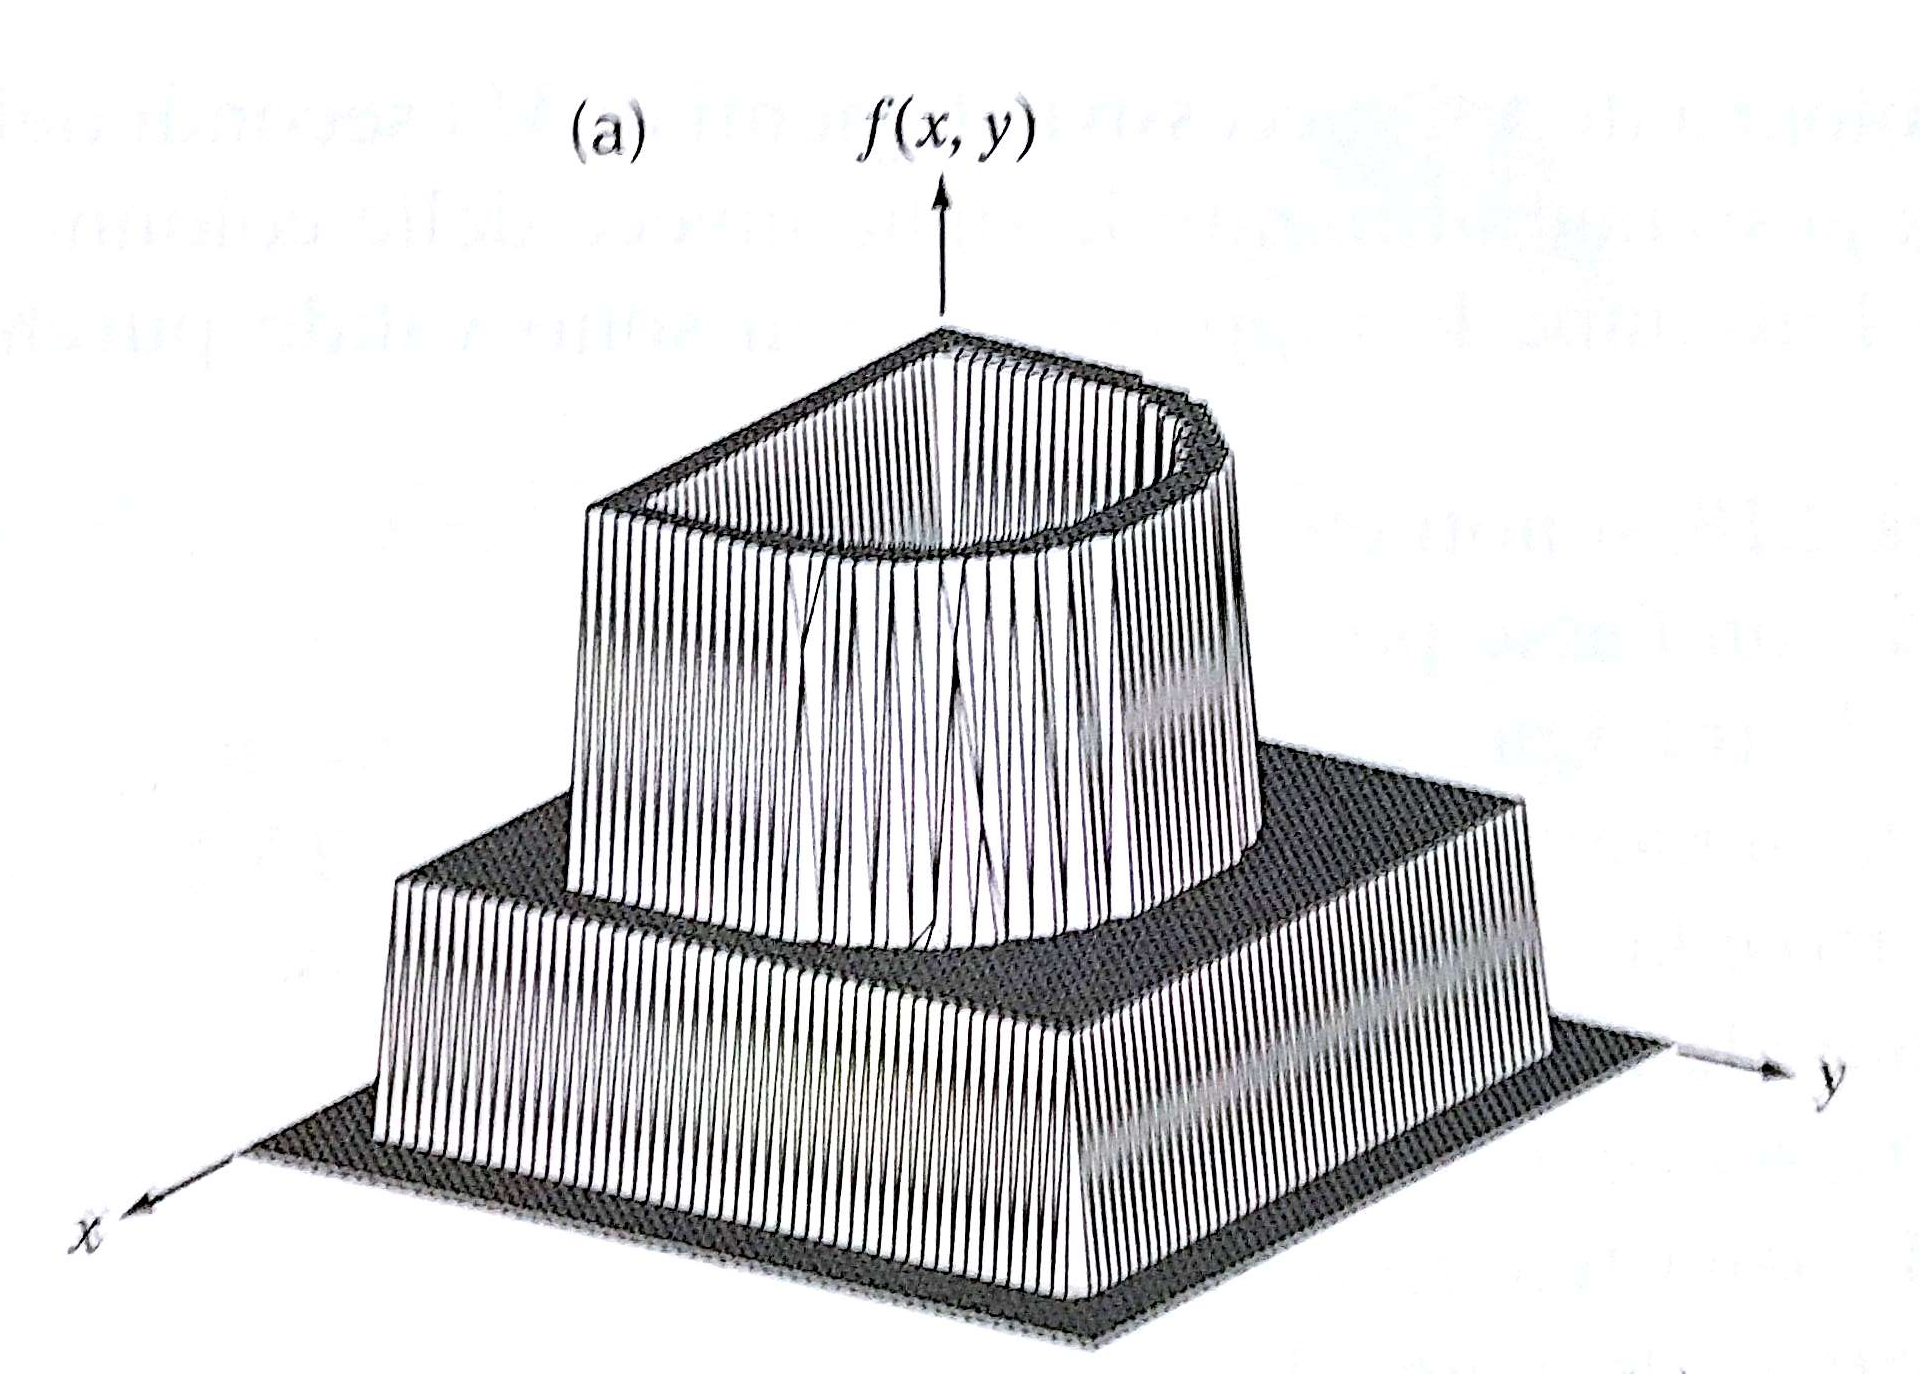
\includegraphics[scale=.15]{img/1050.png}
	\caption{File \protect\url{mission.eps}\label{fig:mission}}
\end{figure}

La segmentazione watershed è utilizzata principalmente per l'estrazione dello sfondo degli oggetti pressoché uniformi (bloblike). Le regioni caratterizzate da piccole variazioni di intensità hanno piccoli valori di gradiente. Per questo motivo si preferisce applicare tale segmentazione al gradiente di una immagine, anziché all'immagine stessa. Nell'esempio che vedremo in seguito, i minimi locali si correlano bene con valori piccoli del gradiente che corrispondono agli oggetti di interesse.

In una topografia consideriamo tre tipi di punti:
\begin{enumerate}
	\item punti appartenenti al minimo locale
	\item punti in cui una goccia d'acqua scorrerebbe verso uno di tali minimi
	\item punti in cui l'acqua potrebbe egualmente cadere in più di un punto di minimo
\end{enumerate}

Per un particolare minimo locale, l'insieme dei punti che soddisfano la condizione 2) è chiamato bacino di raccolta o watershed di questo minimo.

I punti che soddisfano la condizione 3) formano le creste sulla superficie topografica e sono definite linee di divisione o linee di watershed.

Lo scopo dell'algoritmo di segmentazione è quello di trovare le linee di watershed.

Supponiamo che ogni minimo locale venga perforato e che l'intera topografia si riempita dal basso lasciando che l'acqua risalga uniformemente attraverso questi fori.

Quando l'acqua dei differenti bacini rischia di debordare, viene costruita una diga al fine di prevenire tale merging.

L'acqua può raggiungere anche livelli in cui solo le cime di tali dighe risultano visibili. Questi contorni della diga corrispondono alle linee di divisione watershed. Si tratta di contorni connessi estratti dall'algoritmo di segmentazione watershed.

La Fig.10.54 mostra una visualizzazione topografica dell'applicazione dell'algoritmo watershed dove bisogna considerare che:
\begin{itemize}
	\item l'altezza delle "montagne" è proporzionale ai valori di intensità dell'immagine di input
	
	\item per prevenire la crescita del livello dell'acqua oltre i contorni dell'immagine, si chiude il perimetro dell'intera topografia (immagine) con delle dighe che hanno un'altezza maggiore delle montagne, il cui valore viene determinato dal più alto valore possibile di intensità nell'immagine di input
\end{itemize}

\begin{itemize}
	\item si supponga di perforare ogni minimo (le aree in nero in Fig.10.54b) e che l'intera topografia sia sommersa lasciando che il livello dell'acqua risalga da questi buschi a un tasso uniforme
	
	\item la Fig.10.54c mostra un primo livello di inondazione in cui l'acqua (rappresentata in grigio chiaro) ricopre solo le aree che corrispondono allo sfondo nero
	
	\item successivamente, l'acqua risalendo arriva sino ad arrivare rispettivamente al primo e secondo bacino di raccolta (vedi Fig.10.54d e Fig.10.54e)
	
	\item se l'acqua continuasse a salire, questa potrebbe straripare da un bacino all'altro, come accade in Fig.10.54f, dove se non ci fosse una diga (una serie di singoli pixel) l'acqua strariperebbe dal bacino di sinistra a quello di destra
	
	\item in Fig.10.54g l'acqua continua a salire e sono messe in risalto le dighe tra i due bacini e quella in alto del bacino di destra; quest'ultima evita che l'acqua del bacino possa confluire con le aree corrispondenti allo sfondo
	
	\item questo processo continua sino a raggiungere il massimo livello di allagamento corrispondente al valore più alto di intensità dell'immagine
	
	\item la diga finale corrisponde alle linee di watershed, che corrisponde alla segmentazione desiderata come in Fig.10.54h dove si può notare un path di 1 pixel (in nero) sovrapposto all'immagine originale
	
	\item le linee di watershed formano dei path connessi e di conseguenza dei contorni continui tra le regioni
\end{itemize}

\section{L'uso dei marcatori}
L'applicazione diretta dell'algoritmo di segmentazione porta a sovrasegmentazione (oversegmentation) dovuta al rumore o ad altre irregolarità locali del gradiente e questo problema può rendere l'algoritmo di scarsa utilità pratica. Si può migliorare la situazione incorporando una fase di pre-processing (pre-elaborazione) facendo uso per esempio dei marker.

Un marker è una componente connessa appartenente ad una immagine. Si possono avere:
\begin{itemize}
	\item marker interni associati agli oggetti della figura. Una definizione più precisa è:
	\begin{enumerate}
		\item una marker interno è una regione circondata da punti di altitudine elevata
		\item tale che i punti nella regione formino una componente connessa e
		\item in cui tutti i punti della componente connessa abbiamo la stessa intensità
	\end{enumerate}
	
	\item marker esterni associati allo sfondo
\end{itemize}

\subsection{Selezione dei marker}
La tipica procedura per la selezione dei marker consiste di due fasi:
\begin{itemize}
	\item la pre-elaborazione
	\item la determinazione di un insieme di criteri che devono essere soddisfatti dai marker.
\end{itemize}

La selezione del marker può prevedere:
\begin{itemize}
	\item procedure molto semplici basate sui valori di intensità e sulla connettività
	
	\item descrizioni più complesse )
	(dimensione, forma, posizione, distanze relative, tessitura, ecc)
\end{itemize}

L'uso dei marker aggiunge una conoscenza a priori nel processo di segmentazione analoga per certi versi al alcune peculiarità tipiche del sistema visivo umano.

Se consideriamo l'immagine 10.57 noteremo che parte dei problemi sarà dovuta all'eccessiva segmentazione, ovvero di minimi potenziali. A causa della dimensione, molti di questi minimi si riferiscono a dettagli di poco conto. Un metodo efficace per ridurre questo problema, è quello di applicare un filtro di smoothing.

Dopo aver applicato il filtro di smoothing (vedi Fig.10.58a) i marker interni risultanti sono mostrati in grigio chiaro.

In seguito viene applicato l'algoritmo watershed all'immagine con la condizione che \textit{solo} i marker interni siano possibili minimi regionali.

La Fig.10.58a mostra le linee di watershed risultanti e sono definite come marker esterni. Si noti che i punti lungo le linee di watershed passano lungo i punti alti tra i marker vicini.

I marker esterni dividono efficacemente l'immagine in regione, e ognuna di queste contiene un solo marker interno e parte dello sfondo.

A questo punto si possono seguire varie strade:
\begin{itemize}
	\item applicare un qualsiasi algoritmo di segmentazione tra quelli visti in precedenza
	
	\item applicare l'algoritmo di segmentazione ad ogni singola regione. In questo modo si prende in considerazione solo il gradiente dell'immagine e successivamente si applica l'algoritmo solo alle singole watershed che contengono i marker in quella regione.
\end{itemize}

Il risultato finale di buon livello è quello mostrato in Fig.10.58b.